\documentclass{article}

% Language setting
% Replace `english' with e.g. `spanish' to change the document language
\usepackage[english]{babel}

% Set page size and margins
% Replace `letterpaper' with`a4paper' for UK/EU standard size
\usepackage[letterpaper,top=2cm,bottom=2cm,left=3cm,right=3cm,marginparwidth=1.75cm]{geometry}

% Useful packages
\usepackage{amsmath}
\usepackage{graphicx}
\usepackage[colorlinks=true, allcolors=blue]{hyperref}

\DeclareMathOperator*{\argmin}{arg\,min}
\DeclareMathOperator*{\argmax}{arg\,max}

\title{Exploring Hyperparameter Spaces: A Comprehensive Study of Ridge Regularization in Mean-Variance Optimization}
\author{Fernando Urbano}

\begin{document}
\maketitle

\section{Introduction}

Markovitz's construction of the Efficient Frontier in 1952 is among the most significant improvements in quantitative finance and set the start of the Modern Portfolio Theory.

The idea behind the Efficient Frontier provided an algorithm to choose optimal weights for the assets in the portfolios of hedge funds, banks, and other financial institutions.

It is part of the mean-variance optimization framework and served as the foundation for the CAPM theory of Willian Sharpe.

The original algorithm was highly praised for its simplicity accompanied, nonetheless, by a powerful conclusion: portfolio optimization depends on expected returns and risk (measured by variance) and investors aim to maximize expected returns given their levels of risk aversion. With mean-variance optimization, investors can transform their views into investment bets.

With time, the original mean-variance optimization started facing criticism due to estimation error and extremely aggressive allocation as a consequence of mathematical instability. Nowadays, improvements in the field of Machine Learning found paths to mitigate the problem through the use of Regularization (L1 and L2) and Resampling (Monte Carlo and Bootstrapping).

While the original algorithm provides a concise set of hyperparameters, modern applications with regularization techniques require extensive hyperparameter tuning and a gigantic number of possible combinations on how to address the problem. Practitioners often choose one possible set among the vast poll of possibilities, given limited time to train and analyze results.

The goal of our paper is to dive deeper into the tuning of hyperparameters for RIDGE regularization, tirelessly testing possible combinations of different parameters to arrive at general guidelines on how to approach the problem and which sets generate more favorable results.

\section{Methodology}
\subsection{Mean-Variance Optimization}
The optimization process is based on finding the weights for assets in a given portfolio that maximize the expected return of the portfolio given a level of risk or minimize the risk of a portfolio given a level of expected return:

$$
\max_{w} \quad \mu^{T} w \quad \quad
\text{s.t.} \quad w^{T} \Sigma w \leq \sigma^{2}, \quad
\sum_{i=1}^{n} w_{i} = 1
$$

In the equation, $w$ is the vector of weights, $\mu$ is the vector of expected returns, $\Sigma$ is the covariance matrix of the returns, and $\sigma^{2}$ is the tolerated level of risk. The first constraint ensures that the risk of the portfolio is below a certain level, and the second constraint ensures that the investor uses 100\% (not more nor less) of their capital in the allocation.

The Efficient Frontier gives the best allocation for every given risk (variance) level. The curved shape is a consequence of diversification: less than perfect correlation between assets allows for a reduction in the overall risk of the portfolio.

In the picture we highight two points worth of special attention: the Global Minimum Variance Portfolio (GMV), the leftmost point, and the Tangency Portfolio.

\subsection{Global Minimum Variance Portfolio}
The Global Minimum Variance Portfolio (GMV) is the portfolio with the lowest possible variance.

Given the convex nature of the optimization problem, it is possible to find the $w_GMV$ with a closed form solution:

$$
{w}_{\text{GMV}} = \argmin_{w} \quad w^{T} \Sigma w \quad \quad
\text{s.t.} \sum_{i=1}^{n} w_{i} = 1
$$

$$
{w}_{\text{GMV}} = \frac{\Sigma^{-1} \mathbf{1}}{\mathbf{1}^{T} \Sigma^{-1} \mathbf{1}}
$$

In the equation, $\mathbf{1}$ is a vector of ones and $\Sigma^{-1}$ is the inverse of the covariance matrix.

\subsection{Tangency Portfolio}
The Tangency Portfolio is the portfolio that maximizes the Sharpe Ratio, a measure of risk-adjusted return, defined as the ratio of the excess return of the portfolio over the risk-free rate to the standard deviation of the portfolio (square root of the variance):

$$
\text{Sharpe Ratio (SR)} = \frac{\tilde{\mu}^{T} w}{\sqrt{w^{T} \Sigma w}}
$$

Where $\tilde{\mu} = \mu - r_f \mathbf{1}$ is the vector of excess returns, with $r_f$ being the risk-free rate.

Again, given the convex nature of the optimization problem, it is possible to find the $w_{\text{TAN}}$ with a closed form solution:

$$
w_{\text{TAN}} = \argmax_{w} \quad \frac{\mu^{T} w - r_f}{\sqrt{w^{T} \Sigma w}} \quad \quad
\text{s.t.} \sum_{i=1}^{n} w_{i} = 1
$$

$$
w_{\text{TAN}} = \frac{\Sigma^{-1} \tilde{\mu}}{\mathbf{1}^{T} \Sigma^{-1} \tilde{\mu}}
$$

\subsection{Instability and Unpredictability}
The two formulas give us the optimal weights for the given levels of risk. Any other point in the efficient frontier can be obtained by a linear combination of the GMV and the Tangency Portfolio.

$$
w_{\text{optimal}} = \alpha w_{\text{GMV}} + (1 - \alpha) w_{\text{TAN}} \quad \quad \alpha > 0
$$

\begin{figure}[h]
    \centering
    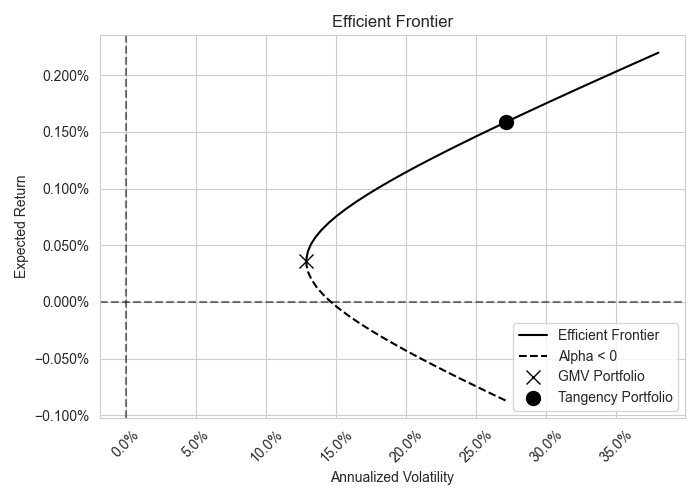
\includegraphics[width=0.8\textwidth]{graphics/report_efficient_frontier.png}
    \caption{Efficient Frontier}
    \label{fig:efficient_frontier}
\end{figure}

However, the expected returns and the covariance matrix are estimated from historical data, and the estimates are subject to error. Returns present small or none autocorrelation, leading to a high degree of unpredictability. The estimates of the covariance matrix are slightly more predictable, but, given the high dimensionality of the problem, small errors in the estimates lead to large errors in optimization and final allocation.

More specifically, the errors are magnified by the $\Sigma^{-1}$ term in the formulas. The inverse of the covariance matrix is highly sensitive to small changes in the estimates, given its high condition number (ratio of the largest to the smallest eigenvalue of the matrix), which serves as a measure of how much the output of the matrix changes due to small changes in the input, and give often highly extreme optimal weights, with large allocations in few assets.

In simpler words, a small difference between the historical and future excess returns ($\tilde{\mu}$) or the covariance matrix ($\Sigma$) lead to a large difference in the optimal weights for the training period and the future period.

\subsection{Ridge Regularization}
Ridge Regularization is a technique used to mitigate the problem of instability in the optimization process. It adds a penalty term to the optimization problem. The point of minimum variance with the new term is called the Regularized Minimum Variance Portfolio (RMVP).

$$
w_{\text{RMVP}} = \argmin_{w} \quad w^{T} \Sigma w + \lambda \|w\|^{2} \quad \quad
\text{s.t.} \sum_{i=1}^{n} w_{i} = 1
$$

The $\lambda$ term is the hyperparameter that controls the trade-off between the variance of the portfolio and the penalty term. As in regression problems, Ridge has the advantage of providing a closed-form solution:

\begin{align*}
w_{\text{RMVP}} = \argmin_{w} & \quad w^{T} \Sigma w + \lambda w^T w \quad \quad \\
                & \quad w^{T} \Sigma w + w^T \lambda I w \quad \quad \\
                & \quad w^{T} (\Sigma + \lambda I) w \quad \quad \\
\end{align*}

The problem is now again a quadratic form, and the solution is:

$$
w_{\text{RMVP}} = \frac{(\Sigma + \lambda I)^{-1} \mathbf{1}}{\mathbf{1}^{T} (\Sigma + \lambda I)^{-1} \mathbf{1}}
$$

The shrinks the optimal weights towards the center of the efficient frontier, reducing the extreme allocations in few assets and decreasing the sensitivity of the optimization process to small changes in the estimates.

In practice, the solution vector $w$ degree of penalty is defined by how much the individual weights differ from the equal weight allocation of of $1/n$, where $n$ is the number of assets in the portfolio.

\begin{figure}[h]
    \centering
    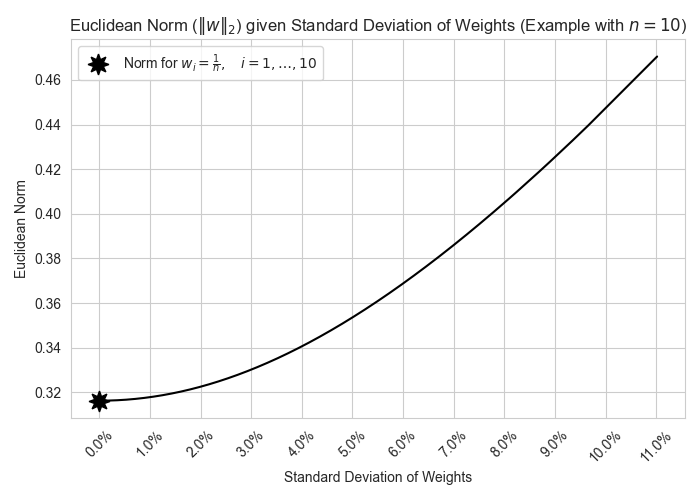
\includegraphics[width=0.8\textwidth]{graphics/report_euclidean_norm.png}
    \caption{Euclidean Norm as a Function of Weights' Standard Deviation}
    \label{fig:euclidean_norm}
\end{figure}

\subsection{Methodology}
In this paper, we explore the hyperparameter space of the RMVP. Using the point of minimum variance steady of the Regularized Tangency Portfolio is viewed as a better approach, given that historical returns are not good predictors of future returns and we intend to remain agnostic about more complicated models on how to predict, given that the focus should remain in the exploration of the hyperparameter of the optimization.

In our tests, we use the conventional format of the regularized optimization problem. Given the selected assets and training data, we use time-series cross-validation to find the optimal $\lambda$ for the RMVP selecting based on the Sharpe Ratio performance. After have choosen the optimal $\lambda$, we calculate the RMVP in the training sample and see their performance in the testing sample.

The hyperparameter space tested is defined by the following parameters:
\begin{itemize}
    \item Choice of number of assets $n$: 5, 10, 12, 17, 30.
    \item Choice of training size $T$ in days: 63, 126, 252, 504.
    \item Choice of testing size $t$ in days (how long the portfolio will run until a new optimization is calculated): 5, 10, 21, 42, 126, 252.
    \item Choice of number of time-series cross-validation $n_{cv}$: 1 to 8.
    \item Choice of cross-validation size $t_{cv}$ as a percentage of the training size: 50\%, 75\%, 100\%, 125\%, 150\%.
\end{itemize}

The $\lambda$'s tested are always in the range of $[0, 3]$, with a step of $0.10$. Before running the simulations, we tested the range in which the optimal $\lambda$'s are found, and limit the search until $3$ given that the optimal is always below this threshold.

Each of 11,200 combinations in the simulation runs from January 1st 2000 to December 31st 2022, totalizing 8.4 million calculations. As a result, we have 11,200 testing portfolios, each with 23 years of data.

The simulations provide answer to questions such:aa
\begin{itemize}
    \item How does the optimal $\lambda$ change with the number of assets?
    \item How does the optimal training size $T$ changes as a function of number of assets and testing size $t$?
    \item What is the optimal number of time-series cross-validation ($n_{cv}$)?
    \item What is the optimal size of the cross-validation ($t_{cv}$)?
    \item How does the distribution of the optimal $\lambda$'s change with the number of assets?
    \item How do moments of financial stress affect the previous questions?
\end{itemize}

The testing portfolios for each of the combinations are aggregated yearly, allowing for comparison of Sharpe Ratio, volatility and returns between the portfolios. The results are analyzed using multivariate ANOVA and visualizations.

\section{Data}
The data is collected from the \hyperlink{https://mba.tuck.dartmouth.edu/pages/faculty/ken.french/data_library.html}{Kenneth French Website}. The website provides daily industry returns in tables dividing the industries in 5, 10, 12, 17, 30, 38, 48, 49 assets from 1926 to 2024 (updated regularly). Each of those tables is used as one of the possible $n$ (number of assets) in the portfolio. The risk-free rate is also provided in the website, inside the "Fama/French 3 Factors" table, and subtract the returns.

\section{How to add Citations and a References List}

\cite{markowitz1952portfolio} or \cite{sharpe1964capital} or \cite{bruder2013regularization}

\bibliographystyle{apalike}
\bibliography{bibliography}

\end{document}